%
% Documentation for the Doubly Link List API.
%
% $Author$
% $Date$
% $Revision$
%
% Compile directive:
%  latex Linklist.tex
%  dvips -t letter Linklist.dvi -o Linklist.ps
%
\documentclass[10pt,letterpaper]{report}

\usepackage{alltt, graphicx}
\pagestyle{plain}
\pagenumbering{arabic}

\begin{document}

\title{A Users Guide for the\\
       Doubly Linked List API\\
       Version 1.1.0}
\author{Carl J. Nobile\\
	cnobile@AppliedTheory.com}
\date{Created: March 28, 1999\\
	Updated: \today}
\maketitle

\chapter*{Preface}
Writing an API for a link list came about after many years of struggling with data storage problems.  I would often write link\-list code embedded in my application, exposing all of its innards to the application.  This was a nightmare to weed through as the application grew in functionality and complexity.  Often much of the functionality that I would have liked in my application would be too difficult to implement or would be kludged in.  If more than one link list was needed my beard would thin.
\vspace{8pt}

\noindent
This manual documents the implementation and use of the Doubly Linked List API.  A brief overview of the design philosophy and how the data is abstracted will be discussed followed by a thorough explanation of the calling and return mechanism of each function.
\vspace{8pt}

\noindent
I hope it is as useful for you as it has been for me.
\vspace{8pt}
\begin{flushright}
Carl J. Nobile\\
April 1999
\end{flushright}

\chapter*{Distribution}
This Doubly Linked List is an Application Programming Interface (API) which can be down loaded from ftp://sunsite.unc.edu/pub/Linux/lib or from me directly at cnobile@AppliedTheory.com.

\chapter*{License}
\begin{center}
\Large			 The "Artistic License"\\
\vspace{8pt}
\Large				Preamble\\
\end{center}
The intent of this document is to state the conditions under which a Package may be copied, such that the Copyright Holder maintains some semblance of artistic control over the development of the package, while giving the users of the package the right to use and distribute the Package in a more-or-less customary fashion, plus the right to make reasonable modifications.
\vspace{8pt}

\noindent
Definitions:
\begin{quote}
"Package" refers to the collection of files distributed by the\linebreak Copyright Holder, and derivatives of that collection of files created through textual modification.

"Standard Version" refers to such a Package if it has not been modified, or has been modified in accordance with the wishes of the Copyright Holder as specified below.

"Copyright Holder" is whoever is named in the copyright or copyrights for the package.

"You" is you, if you're thinking about copying or distributing this Package.

"Reasonable copying fee" is whatever you can justify on the basis of media cost, duplication charges, time of people involved, and so on.  (You will not be required to justify it to the Copyright Holder, but only to the computing community at large as a market that must bear the fee.)

"Freely Available" means that no fee is charged for the item itself, though there may be fees involved in handling the item.  It also means that recipients of the item may redistribute it under the same conditions they received it.
\end{quote}

\noindent
1. You may make and give away verbatim copies of the source form of the Standard Version of this Package without restriction, provided that you duplicate all of the original copyright notices and associated disclaimers.
\vspace{8pt}

\noindent
2. You may apply bug fixes, portability fixes and other modifications derived from the Public Domain or from the Copyright Holder.  A Package modified in such a way shall still be considered the Standard Version.
\vspace{8pt}

\noindent
3. You may otherwise modify your copy of this Package in any way, provided that you insert a prominent notice in each changed file stating how and when you changed that file, and provided that you do at least ONE of the following:

\begin{quote}
(a) place your modifications in the Public Domain or otherwise make them Freely Available, such as by posting said modifications to Usenet or an equivalent medium, or placing the modifications on a major archive site such as uunet.uu.net, or by allowing the Copyright Holder to include your modifications in the Standard Version of the Package.

(b) use the modified Package only within your corporation or organization.

(c) rename any non-standard executables so the names do not conflict with standard executables, which must also be provided, and provide a separate manual page for each non-standard executable that clearly documents how it differs from the Standard Version.

(d) make other distribution arrangements with the Copyright Holder.
\end{quote}

\noindent
4. You may distribute the programs of this Package in object code or executable form, provided that you do at least ONE of the following:

\begin{quote}
(a) distribute a Standard Version of the executables and library files, together with instructions (in the manual page or equivalent) on where to get the Standard Version.

(b) accompany the distribution with the machine-readable source of the Package with your modifications.

(c) give non-standard executables non-standard names, and clearly document the differences in manual pages (or equivalent), together with instructions on where to get the Standard Version.

(d) make other distribution arrangements with the Copyright Holder.
\end{quote}

\noindent
5. You may charge a reasonable copying fee for any distribution of this Package.  You may charge any fee you choose for support of this Package.  You may not charge a fee for this Package itself.  However, you may distribute this Package in aggregate with other (possibly commercial) programs as part of a larger (possibly commercial) software distribution provided that you do not advertise this Package as a product of your own.  You may embed this Package's interpreter within an executable of yours (by linking); this shall be construed as a mere form of aggregation, provided that the complete Standard Version of the interpreter is so embedded.
\vspace{8pt}

\noindent
6. The scripts and library files supplied as input to or produced as output from the programs of this Package do not automatically fall under the copyright of this Package, but belong to whomever generated them, and may be sold commercially, and may be aggregated with this Package.  If such scripts or library files are aggregated with this Package via the so-called "undump" or "unexec" methods of producing a binary executable image, then distribution of such an image shall neither be construed as a distribution of this Package nor shall it fall under the restrictions of Paragraphs 3 and 4, provided that you do not represent such an executable image as a Standard Version of this Package.
\vspace{8pt}

\noindent
7. C subroutines (or comparably compiled subroutines in other languages) supplied by you and linked into this Package in order to emulate subroutines and variables of the language defined by this Package shall not be considered part of this Package, but are the equivalent of input as in Paragraph 6, provided these subroutines do not change the language in any way that would cause it to fail the regression tests for the language.
\vspace{8pt}

\noindent
8. Aggregation of this Package with a commercial distribution is always permitted provided that the use of this Package is embedded; that is, when no overt attempt is made to make this Package's interfaces visible to the end user of the commercial distribution.  Such use shall not be construed as a distribution of this Package.
\vspace{8pt}

\noindent
9. The name of the Copyright Holder may not be used to endorse or promote products derived from this software without specific prior written permission.
\vspace{2pt}

\noindent
10. THIS PACKAGE IS PROVIDED "AS IS" AND WITHOUT ANY EXPRESS OR IMPLIED WARRANTIES, INCLUDING, WITHOUT LIMITATION, THE IMPLIED WARRANTIES OF MERCHANTABILITY AND FITNESS FOR A PARTICULAR PURPOSE.

\begin{center}
The End
\end{center}

\chapter*{Introduction}
There are many goals to achieve when deciding to write an API.  The functions in the library should be reenterable, easy to include in an application, platform independent, and reasonably flexible with enough functionality to be usable.  These goals can often be contradictory; however, they are achievable with enough forethought and planning.
\vspace{8pt}

\noindent
This package is sufficiently abstracted so that the programmer will neither need to know or care how it is implemented.  At least that is the goal I have striven to achieve while writing it.
\vspace{8pt}

\noindent
Within this package is found the: source files written in C; make files for various platforms and compilers; text script which sets the environment correctly when it runs the demo program created by the make utility; README, INSTALL, and HISTORY text files; Artistic license; and the documentation in \LaTeXe form.
\vspace{8pt}

\noindent
A short overview, will follow, discussing the philosophy of how the package works including a rational of the structure and type definition use in the package.
\vspace{8pt}

\noindent
Then the library itself is broken into six groups: initialization, status, data manipulation, pointer manipulation, search, and input/output.

\begin{quote}
(a) The initialization group handles the creation, initializing, and destruction of the link list.

(b) The status group returns various kinds of information about the status of the link list during its operation.

(c) The pointer manipulation group allows the positioning of the current pointer to the head, tail or to an arbitrary node within the list.

(d) The data modification group adds and deletes nodes.

(e) The search group returns the record information based on key data or on the absolute record position.

(f) The input/output group saves or retrieves record data to or from a disk file.
\end{quote}

\noindent
At this writing there are 29 functions in the library, each one of which is thoroughly explained and examples given when needed.

\chapter*{Overview}
When writing tools such as this, one needs to be concerned with how it affects the entire programming environment.  One of the most important aspects of this environment is the problem concerning \emph{namespace} pollution.  To minimize this problem I have used DLL\_ as a prefix to all function names and enumerated \texttt{typedef}s.
\vspace{8pt}

\noindent
It is often the case that search criteria will remain the same between quiries.  As such a state table is implimented that passes the current state to the search functions.  There are two functions one to set and the other to read the state table.







\chapter*{Structures}
Most implementations of link lists allocate a single node per record and these nodes are what are linked to each other.  This type of algorithm works well when the link list is embedded in the application code, but not when implementing a link list within an API, because it cannot be made reenterant.
\vspace{8pt}

\noindent
A well written Application Programming Interface (API) requires that the functions contained within it be reenterant and also creates an environment where the code can be abstracted.  In order to take advantage of these two ideas the Doubly Linked List (hereafter referred to as the DLL) has a three level hierarchy.  The first level we will refer to as the 'Top Level Struct'.  All the global data is held by one of these structures and it is allocated once for each incident of the link list.  

%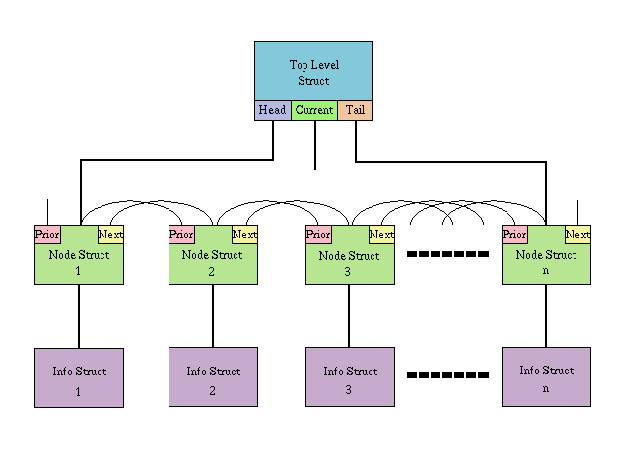
\includegraphics[width=5in]{linklistDiagram.gif}

\small
\begin{alltt}
typedef struct list
   \{
   Node           *head;         /* pointer to head record */
   Node           *tail;         /* pointer to tail record */
   Node           *current;      /* pointer to current record */
   Node           *saved;        /* pointer to stored record */
   size_t         infosize;      /* size of record incident */
   unsigned long  listsize;      /* number of records in list */
   unsigned long  current_index; /* index value of current record */
   unsigned long  save_index;    /* index value of stored record */
   DLL_Boolean    modified;      /* modified flag (TRUE or FALSE) */
   DLL_SrchOrigin search_origin; /* location a search originates from */
   DLL_SrchDir    search_dir;    /* direction the search proceeds from */
   \} List;
\end{alltt}
\normalsize
\vspace{8pt}

\noindent
At the next level is the 'Node Struct'.  This structure holds the pointer to the actual record data plus the pointers to the next and prior nodes.  It is allocated once for each record structure.

\small
\begin{alltt}
typedef struct node
   \{
   Info        *info;     /* pointer to record data */
   struct node *next;     /* pointer to next node */
   struct node *prior;    /* pointer to prior node */
   \} Node;
\end{alltt}
\normalsize
\vspace{8pt}

\noindent
The third and final level is the 'Info Struct', which holds the actual data inserted by the application.  The Info Struct is defined by the developer and is only restricted by the environment in which the application runs or is compiled in.

\small
\begin{alltt}
typedef struct your_info
   \{
   type your_data;        /* Your data goes here */
   \} YourInfo;
\end{alltt}
\normalsize
\vspace{8pt}

\noindent
There is one more structure which is not part of this hirarchy.  It is only used to return the current state of the search criteria.

\small
\begin{alltt}
typedef struct search_modes
   \{
   DLL_SrchOrigin search_origin; /* Search from head, tail, or current */
   DLL_SrchDir    search_dir;    /* Search up or down */
   \} DLL_SearchModes;
\end{alltt}
\normalsize

\chapter*{Enumerations}
I'm a firm believer that the return values of functions should be predefined \texttt{typedef} enumerations.  There are two reasons for this.  The first is that many compilers will complain when a switch statement is used to test the return values of functions with one or more of the enumerated values missing thus alerting the developer to using the \texttt{default} statement.   The second reason is that the \texttt{typedef} name can be used as the return type of the function disallowing anything other than the enumerated values to be returned.  These are good things and should be taken advantage of.
\vspace{8pt}

\noindent
Since, that at the time of this writing Booleans are not part of the C specifications I've created my own.

\small
\begin{alltt}
typedef enum
   \{
   DLL_FALSE,
   DLL_TRUE
   \} DLL_Boolean;
\end{alltt}
\normalsize
\vspace{8pt}

\noindent
Many functions return the \texttt{typedef} enumerated type DLL\_Return as shown below.

\small
\begin{alltt}
typedef enum
   \{
   DLL_NORMAL,            /* normal operation */
   DLL_MEM_ERROR,         /* malloc error */
   DLL_ZERO_INFO,         /* sizeof(Info) is zero */
   DLL_NULL_LIST,         /* List is NULL */
   DLL_NOT_FOUND,         /* Record not found */
   DLL_OPEN_ERROR,        /* Cannot open file */
   DLL_WRITE_ERROR,       /* File write error */
   DLL_READ_ERROR,        /* File read error */
   DLL_NOT_MODIFIED,      /* Unmodified list */
   DLL_NULL_FUNCTION      /* NULL function pointer */
   \} DLL_Return;
\end{alltt}
\normalsize
\vspace{8pt}

\noindent
The next two enumerations are used to determine the state of search inquiries, one is used to determine the origin and the other for the direction.  These values are passed as arguments to the \texttt{DLL\_SetSearchModes()} function.

\small
\begin{alltt}
typedef enum
   \{
   DLL_ORIGIN_DEFAULT,    /* Use current origin setting */
   DLL_HEAD,              /* Set origin to head pointer */
   DLL_CURRENT,           /* Set origin to current pointer */
   DLL_TAIL               /* Set origin to tail pointer */
   \} DLL_SrchOrigin;

typedef enum
   \{
   DLL_DIRECTION_DEFAULT, /* Use current direction setting */
   DLL_DOWN,              /* Set direction to down */
   DLL_UP                 /* Set direction to up */
   \} DLL_SrchDir;
\end{alltt}
\normalsize
\vspace{8pt}

\noindent
The last enumerated type is used to determine the direction of inserting and swaping a record and is passed as an argument to two functions\linebreak \texttt{DLL\_InsertRecord()} and \texttt{DLL\_SwapRecord()}.

\small
\begin{alltt}
typedef enum
   \{
   DLL_INSERT_DEFAULT,    /* Use current insert setting */
   DLL_ABOVE,             /* Insert new record ABOVE current record */
   DLL_BELOW              /* Insert new record BELOW current record */
   \} DLL_InsertDir;
\end{alltt}
\normalsize

\chapter*{Functions}
The function calls below are grouped by their general function as described above.  They are written in manpage style so that I only have to document the API once.

\section*{Initialization}
\begin{description}
\item[NAME]\hspace{1em}\\
DLL\_CreateList, DLL\_InitializeList, DLL\_DestroyList, --- initializing group
\item[SYNOPSIS]
\begin{alltt}\hspace{1em}
#include <linklist.h>

DLL_CreateList(List **name);
DLL_InitializeList(List *list, size_t infosize);
DLL_DestroyList(List **name);
\end{alltt}
\item[DESCRIPTION]\hspace{1em}\\






\end{description}
\end{document}
